\documentclass{article}%
\usepackage[T1]{fontenc}%
\usepackage[utf8]{inputenc}%
\usepackage{lmodern}%
\usepackage{textcomp}%
\usepackage{lastpage}%
\usepackage[head=40pt,margin=0.5in,bottom=0.6in]{geometry}%
\usepackage{graphicx}%
%
\title{\textbf{Siete consejos para evitar que las aplicaciones roben tus datos}}%
\author{GDA| EL COMERCIO| PERÚ}%
\date{04/03/2019}%
%
\begin{document}%
\normalsize%
\maketitle%
\textbf{URL: }%
http://www.el{-}nacional.com/noticias/ciencia{-}tecnologia/siete{-}consejos{-}para{-}evitar{-}que{-}las{-}aplicaciones{-}roben{-}tus{-}datos\_273309\newline%
%
\textbf{Periodico: }%
EN, %
ID: %
273309, %
Seccion: %
Ciencia y Tecnología\newline%
%
\textbf{Palabras Claves: }%
Ciencia y Tecnología\newline%
%
\textbf{Derecho: }%
2.1%
, Otros Derechos: %
\newline%
%
\textbf{\textit{En los últimos años, muchas aplicaciones han sido expuestas como~malware, las cuales son usadas para cometer fraude y extraer información confidencial}}%
\newline%
\newline%
%
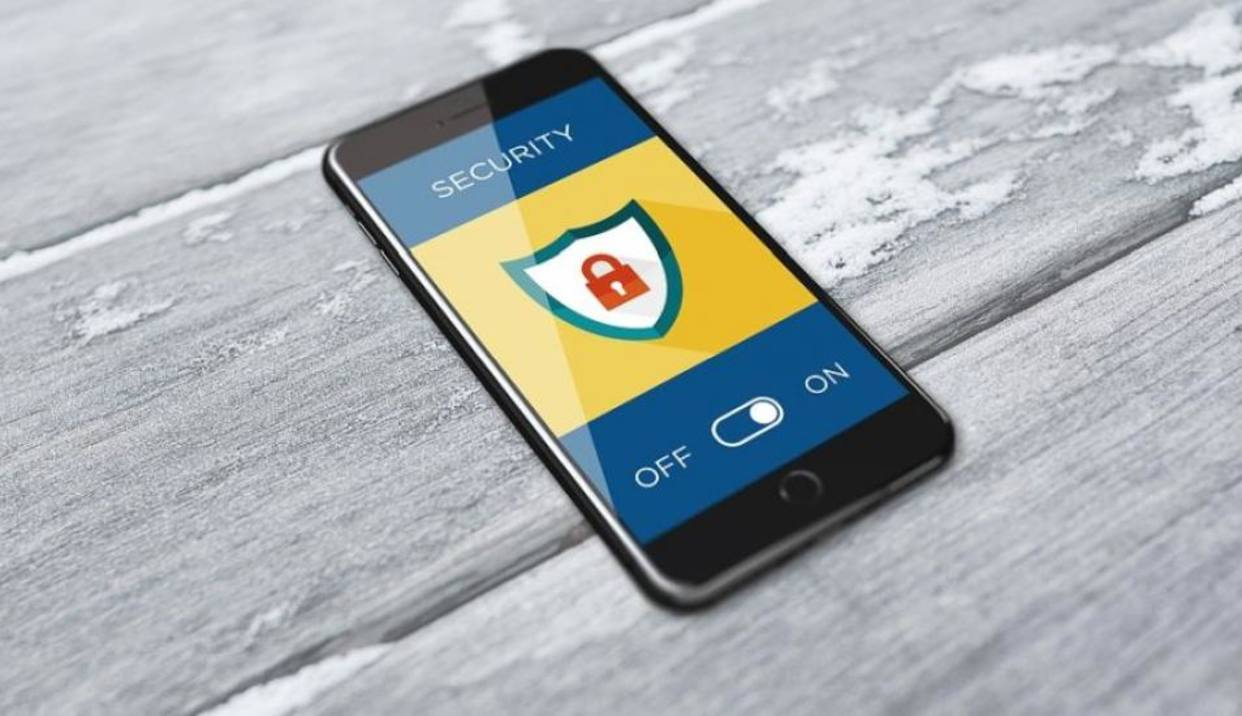
\includegraphics[width=300px]{EN_273309.jpg}%
\newline%
%
Frecuentemente rebotan noticias sobre cómo la~información personal~de muchos usuarios ha estado en peligro luego de una filtración de datos, y como las aplicaciones forman parte de este problema. En los últimos años, muchas aplicaciones han sido expuestas como~malware, las cuales son usadas para cometer fraude y extraer información confidencial.%
\newline%
%
No existe una forma de saber si una aplicación tiene planes para recopilar nuestros datos. Por ello, es recomendable seguir estos conejos para que los usuarios protejan sus datos personales al utilizar aplicaciones.%
\newline%
%
1. Utilizar un administrador de contraseñas%
\newline%
%
Tener una contraseña segura es el primer paso para mantener a salvo los datos personales. Combinar letras y números es una buena opción, así será menos probable que los hackers la logren descifrar.%
\newline%
%
Si no tienes ideas, usar una aplicación de administración de contraseñas resulta útil, porque crean una diseñada para los usuarios.~Asimismo, es mejor evitar usar la misma contraseña en varias cuentas, porque así será más difícil que si encuentran una cuenta, ingresen a las demás.%
\newline%
%
2. Utilizar VPN en Wi{-}Fi público%
\newline%
%
Usar una red privada virtual (VPN por sus siglas en inglés) es importante cuando se está en una red Wi{-}Fi pública para mantener los datos seguros.%
\newline%
%
La VPN evita que otras personas que se esconden en la red pública espíen la información de un usuario. También permite enmascaras las transmisiones de datos, evitar el filtrado y censura de Internet y acceder a una mayor variedad de contenido.%
\newline%
%
3. Tomar en cuenta los permisos y accesos%
\newline%
%
Es necesario hacer una doble verificación de los permisos que se solicitan para las aplicaciones.%
\newline%
%
"Si otorgas permiso a una aplicación para que acceda a tu lista de contactos, datos de GPS, imágenes, o cualquier otra información, debes asumir que está usando esos datos", indicó Ray Walsh, un experto en privacidad digital en BestVPN.com. "Verifica siempre todos los permisos durante la instalación y anula tantos permisos como sea posible en la configuración de tu dispositivo", agregó.%
\newline%
%
También es bueno saber si tiene sentido que una aplicación solicite ciertos permisos. Por ejemplo, si una app necesita datos que no son relevantes para su funcionamiento, es una señal.%
\newline%
%
4. Investiga la aplicación o desarrolladora%
\newline%
%
Una búsqueda en Google puede ayudar al usuario a comprender mejor si una aplicación es segura. Se recomienda buscar el nombre de la aplicación junto a la frase “data scandal” o “scam”.%
\newline%
%
Es aconsejable evitar una aplicación si es la única producida por un desarrollador o si el desarrollador ha sido responsable de una app sospechosa.%
\newline%
%
5. Reducir la exposición en redes sociales%
\newline%
%
Se recomienda limitar la cantidad de información que se comparte en las redes sociales. Cuanta más información se cague, más datos estarán disponibles para crear anuncios hacia ti.%
\newline%
%
Es necesario ingresar solo la cantidad mínima de información y no agregar datos adicionales para completar el perfil.%
\newline%
%
6. Actualiza el software del sistema operativo%
\newline%
%
Es importante tomarse el tiempo para actualizar el sistema operativo del celular. Tener al día las actualizaciones puede mantener más seguro el dispositivo como los datos del usuario.%
\newline%
%
También es bueno ajustar la configuración del teléfono para que se actualice de manera automática.%
\newline%
%
7. Descargar aplicaciones solo del Play Store y App Store%
\newline%
%
Si bien no todas las aplicaciones de las tiendas de Google y Apple son 100\% confiables, se recomienda solo descargarlas desde estos sitios.~La ventaja es que estas son analizadas para garantizar que cumplan con la calidad estándar de protección de datos y también se les exige que tengan políticas de privacidad.%
\newline%
%
Evitar también descargar una aplicación de una fuente de dudosa reputación, pues aumenta los riesgos para el dispositivo y datos personales.%
\newline%
%
\end{document}